%\documentclass[a4paper]{article}
\documentclass[17pt]{extarticle}
\usepackage{polyglossia}
\usepackage[margin=10mm]{geometry}
\setdefaultlanguage{marathi}
\setotherlanguages{english}
\setmainfont[Mapping=velthuis-sanskrit,Script=Devanagari,Language=Sanskrit]{Noto Serif Devanagari}
%\setmainfont[Mapping=velthuis-sanskrit,Script=Devanagari,Language=Sanskrit]{Sanskrit2003}
%\setmainfont[Mapping=velthuis-sanskrit,Script=Devanagari,Language=Sanskrit]{Shobhika}
\newfontfamily\englishfont{Noto Serif}
%\newfontfamily\sanskritfont[Mapping=velthuis-sanskrit,Script=Devanagari,Language=Sanskrit]{Noto Serif Devanagari}
% make sure ~ as non-breaking space doesn't interfere with velthuis-sanskrit mapping
\edef~{\string~}
\pagenumbering{gobble}
\setlength{\parindent}{0pt}% Remove paragraph indent
\usepackage[skip=\medskipamount]{parskip}
\usepackage{xcolor}
\usepackage{graphicx}
\usepackage{hyperref}
\hypersetup{
    colorlinks=true,
    linkcolor=blue,
    filecolor=magenta,
    citecolor=blue,
    urlcolor=purple,
}
\newcommand \eng[1]{
    \textenglish{#1}
}

% control hyphenation: https://tex.stackexchange.com/a/177179/64425
\tolerance=1
\emergencystretch=\maxdimen
\hyphenpenalty=10000
\hbadness=10000
% control hyphenation: https://tex.stackexchange.com/a/177179/64425

\begin{document}

\title{ra.mga maajhaa vegaLaa -- eka prayoga}
\author{sigmaa-vana-vaasii ``\eng{Black-Box}''}
\date{sap.te.mbar 2022}
\maketitle
%\hrule
%\vspace{5mm}
%\vspace{5mm}
%\hrule
\let\thefootnote\relax\footnotetext{\eng{version: 0.7}}
\newpage
sarvaprathama, kaahii suucanaa, aapalyaa sarvaa.msaa.thiica --
\begin{enumerate}
    \item paara.mpaarika pratyak.sa (\eng{live}) naa.takaaca.m jasa.m skrip.t asata.m tasa.m he naahiiye. 
    \item haa prayoga aapa.na pratyak.sa kara.naara naahiica aahota; aapa.na sagaLyaa.mniica yaatiila vegavegaLe bhaaga, aapaapalyaa aava.diinusaara, aapalyaa gharii ``\eng{video shoot/audio recording}'' kara.naara aahota. aa.ni maga te bhaaga ekatra sa.mpaadita (\eng{edit}) hotiila aa.ni ek \eng{MP4} phaaiil tayaara hoiila. sa.mpaadana (\eng{editing}) sopa.m jaava.m mha.nuuna pratyeka \eng{video/audio file} laa eka vi"si.s.ta naava de.nyaata aala.m aahe.
    \item nivedana kara.naaraa suutradhaara jarii asalaa tarii te paatra aapa.na sagaLeca ra.mgava.naara aahota. mha.naje amuka eka ja.na suutradhaara nasela (jarii skrip.t madhye ``suutradhaara'' asa.m mha.nalela.m asela), pratyeka suutradhaaraace naava tyaa-tyaa .thikaa.nii ka.msaata dilele asela.
    \item skrip.t madhye \eng{(note:)} asa.m lihuuna \eng{video editor} laa kaahii suucanaa kelyaa aaheta.
\end{enumerate}
\newpage

skriin vara khaaliila pratimaa ujaLate \dots

\begin{center}
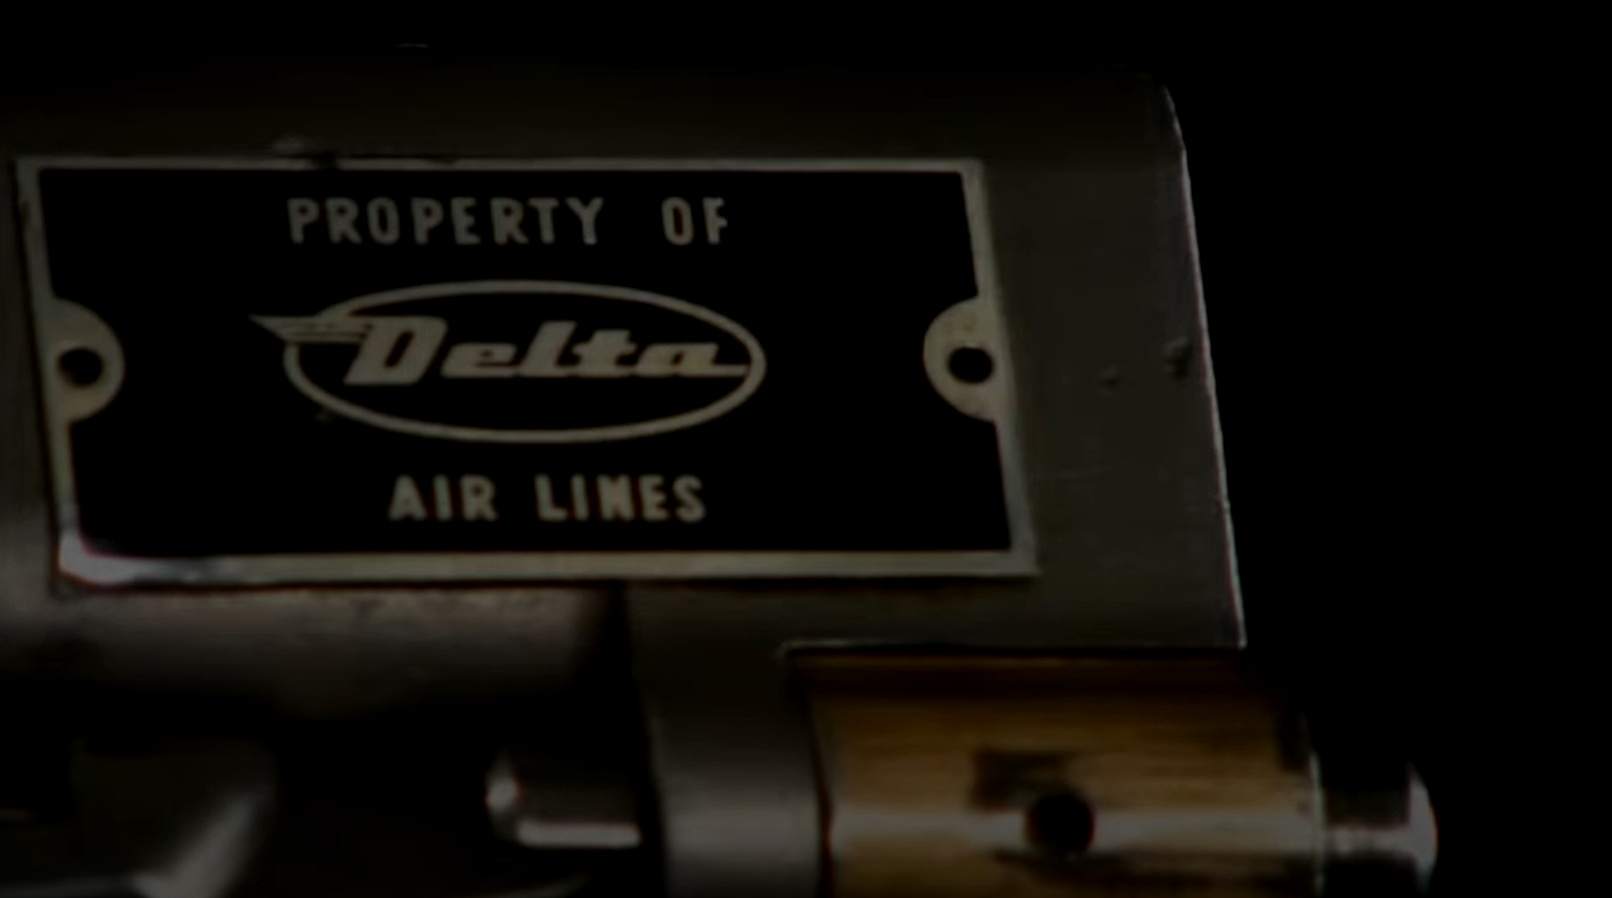
\includegraphics[width=1.0\textwidth]{img/black-box-1}
\end{center}
(yaa paar"svabhuumiivara) \textbf{suutradhaara ()}: (a.mdhaaraata, phakta ga.mbhiira aavaajaata) namaskaara ma.m.daLii, namaskaara. naahii, tumhaalaa mii disata naahiiye ajuuna, pa.na yaacaa artha mii ithe naahiiye asaa naahii. je disata.m teca asata.m asaa .rgvedaatalyaa ``cak.survai satyam'' yaa "srutiicaa artha aahe, pa.na a"saa kitiitarii go.s.tii aaheta kii jyaa kadaacita disata naahiita, pa.na tyaa asataata, aa.ni itaka.mca navhe tara tyaa prasa.mgii aapalyaa sagaLyaata jaasta upayogii pa.dataata.

(\eng{note: lights on!})

\textbf{suutradhaara ()}:
aataa heca pahaa naa -- he kasala.m citra aahe? yaaca.m khara.m naava aahe, \eng{Foil Oscillographic Recorder}. 

go.mdhaLalaata naa? vaa.tala.mca malaa. pa.na hava.m tara aapalyaa \eng{Bill Hammack} yaa siddhahasta ta.mtraj~naalaa vicaaruyaa he kaaya aahe mha.nuuna. 

(\eng{note:} ithe \eng{https://youtu.be/xlY5W7be5jU?t=65} haa vhi.di{}o (barobara yaaca \eng{timestamp} laa) caaluu vhaayalaa havaa aa.ni saadhaara.na 10 seka.mda caaluu rahaayalaa havaa.)

barobara, haa aahe aapalaa \eng{Flight Data Recorder} arthaata \eng{``black box''}! ko.natyaahii vimaanaata ki.mvaa mo.th.thyaa jahaajaata haa basavalelaa asato. tumhaalaa maahitii aselaca kii yaaca.m kaama ekaca -- je kaahii gha.dala.m te mudrita karuuna .thevaayaca.m. mha.naje kaahii apaghaata vagaire jhaalaaca, tara nakkii kaaya gha.dala.m yaacii eka no.mda tyaacyaaka.de asate tii paahuuna tasaa apaghaata punhaa ho.naara naahii yaacii kaaLajii ghetaa yete. ekaa d.r.s.tiine itihaasakaaraca jhaalaa haa \eng{black box}, naahii kaa?

"sivaaya ${1000}^\circ$ selsiyas eva.dha.m taapamaana aa.ni svata.hcyaa vajanaacyaa 3400 pa.ta vajana sahana kara.nyaacii yaacii k.samataa asate! kaahii jhaala.m tarii haa abaadhita raahuu "sakela asa.m yaaca.m \eng{design} asata.m. mha.naje yaa na"svara jagaata toca kaaya to eka.taa avinaa"sii!

\textbf{suutradhaara ()}: hii jhaalii \eng{black box} cii ``taa.mtrika baajuu''. pa.na svaatiilaa jaa.naavalii tii tyaacii kaavyaatma, tarala baajuu:
(\eng{note: Swati recites her poem})


\begin{center}
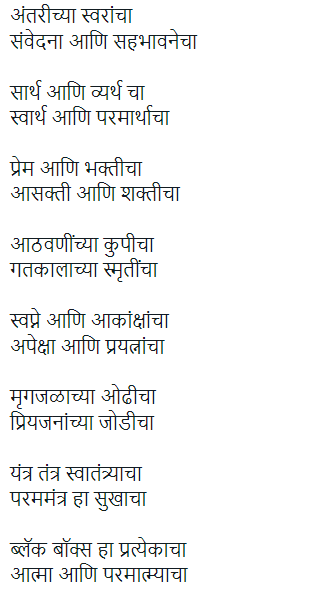
\includegraphics[width=0.3\textwidth]{img/black-box-poem-swati}
\end{center}

aa.ni mha.nuunaca he naava aamhii aamacyaa .tiima saa.thii niva.dala.m. 

\textbf{suutradhaara ()}: a"saa yaa anivaarya \eng{black box} 

\begin{center}
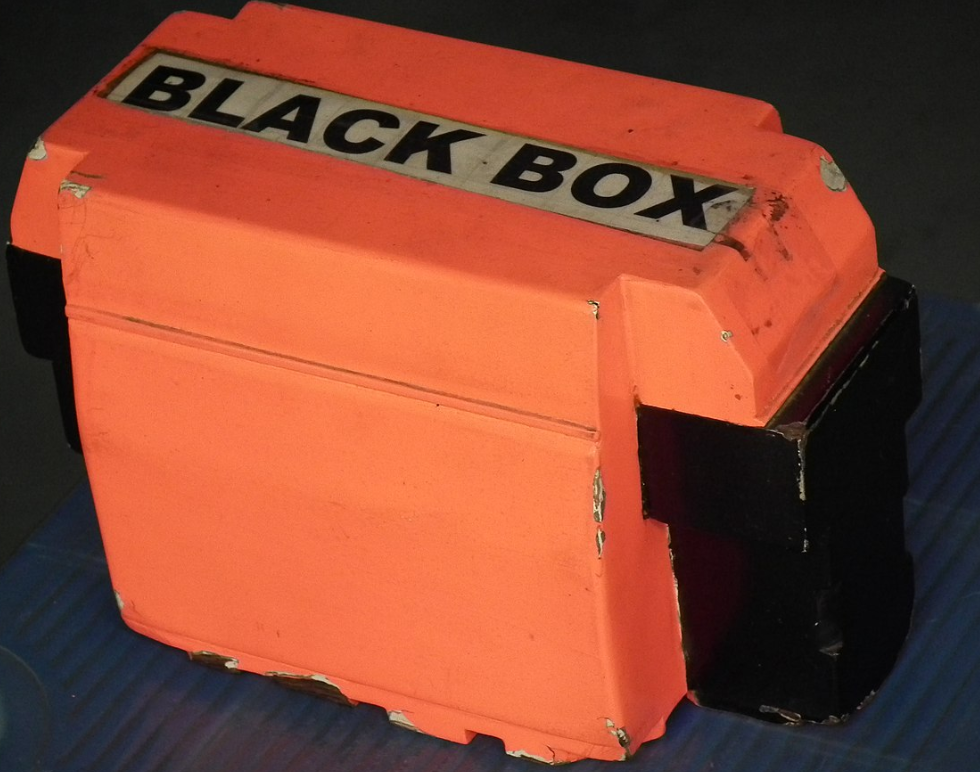
\includegraphics[width=0.3\textwidth]{img/orange}
\end{center}

cii aa.nakhii eka ga.mmata mha.naje yaacaa ra.mga maatra asato ke"sarii. kaara.na kaaya, tara taa.mba.daa (\eng{note: red color can flash in the background on the right}) aa.nii pivaLaa (\eng{note: yellow color can flash in the background on the left}) yaa agadii saamaanya ra.mgaa.mpaasuuna tayaara jhaalelaa haa asaamaanya ke"sarii ra.mga khuupa laa.mbavaruunahii disuu "sakato! 
(\eng{note: merge the two colors in the background to show a fluorescent orange Flight Data Recorder.})

\textbf{suutradhaara ()}: aa.ni yaa ke"sarii ra.mgaacaa dimaakha kaaya var.naavaa! ugavatiicyaa suuryaacaa, maavaLatiicyaa .dhagaa.mcaa, i.mdradhanu.syaatalaa, ge.m.dedaara jhe.m.duucyaa phulaa.mcaa, naajuuka praajaktaacyaa phulaa.mcyaa de.thaa.mcaa, yogii vyakticyaa vastraa.mcaa, saLasaLatyaa caitanyaacaa, tejaacaa, "sauryaacaa, aa.ni adhyaatmikatecaa haa bahaaradaara var.na! 

baakiibaaba borakara aaja asate tara tyaa.mnii mha.tala.m asata.m -- 

\begin{center}
ase naanaagu.nii naari.mge

kitii saa.mguu tyaa.mce laLe \dots
\end{center}

\textbf{suutradhaara ()}: divasaacii suravaataca hote muLii te suuryabi.mba praaciivaratii umalalyaane aa.ni ni"secaa tama saralyaane. agadii aapalyaa laa.dakyaa pii. saavaLaaraamaa.mcyaa "sabdaa.mta, pa.m. h.rdayanaathaa.mcyaa svarasaajaata, aa.ni aa"saataaii.mcyaa ajaraamara, navhe, diipaacyaa aavaajaata aikaa \dots 

(\eng{note: playback/video of the song from dharmakanyaa})


\begin{center}
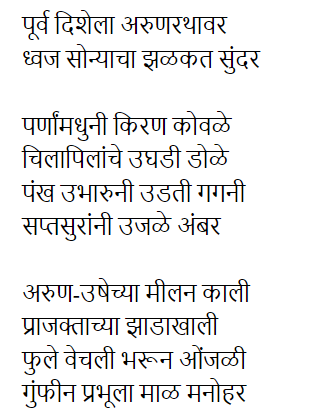
\includegraphics[width=0.3\textwidth]{img/puurva-dishelaa}
\end{center}

\textbf{suutradhaara ()}: nisargaata aneka .thikaa.nii disa.naaraa haa ke"sarii var.na aamacyaa .tiima cyaa bodhacinha mha.naje \eng{logo} madhye suddhaa aahe. yaa aamacyaa mitra-maitri.nii.mnii asa.m kela.m aamaca.m he bodhacinha tayaara\dots

\eng{(note: Insert a story/video of making of the logo.)}

\eng{(note: Perhaps we should also insert the war cry here, although I am not yet sure how to weave it in the story.)}

\textbf{suutradhaara ()}: tara asaa haa ke"sarii disa.naaraa \eng{black box}. pa.na ra.mgaa.mca.m jaga kaaya, sagaLa.mca vilobhaniiya! pratyekaacii .teva-.theva vegaLii, vegavegaLyaa paddhatiine aakar.saka. 

aa.ni\dots aa.ni aapalyaa sagaLyaa.mca.m tarii kaaya! mo.thii ga.mmata aahe naahii? aapalyaatalaa pratyeka ja.na ekaa svata.mtra pariine eka \eng{black box}! pratyekaace a.mtara.mga vegaLe. punhaa ekadaa borakaraa.mcyaa "sabdaa.mta saa.mgaayaca.m jhaala.m tara --

\begin{center}
jii jii ugave caa.mda.nii

ticyaa pariine dekha.nii
\end{center}

yaa sigmaa vanaatalyaa ga.ne"sotsavaacyaa ruupaane hota asalelaa, dona var.saa.mcii diirgha kaaLaraatra saralyaana.mtaracaa haa ke"sarii, navhe, sonerii u.sa.hkaala mha.naje maanavii manaacyaa utka.tatecaa mahotsava! a"sii aneka maanavii mana.m aana.mdaane ekatra yetaata, gu.nyaagovi.mdaane naa.mdataata, aa.ni aayu.syaaca.m sona.m hota.m.

a"saa yaa athaa.mga, anaakalaniiya, \eng{black box} saarakhyaa manaacaa ra.mga tarii ko.nataa? kavivarya sure"sa bha.taa.mnii manoj~na "sabdaa.mta mha.tala.mya --

\begin{center}
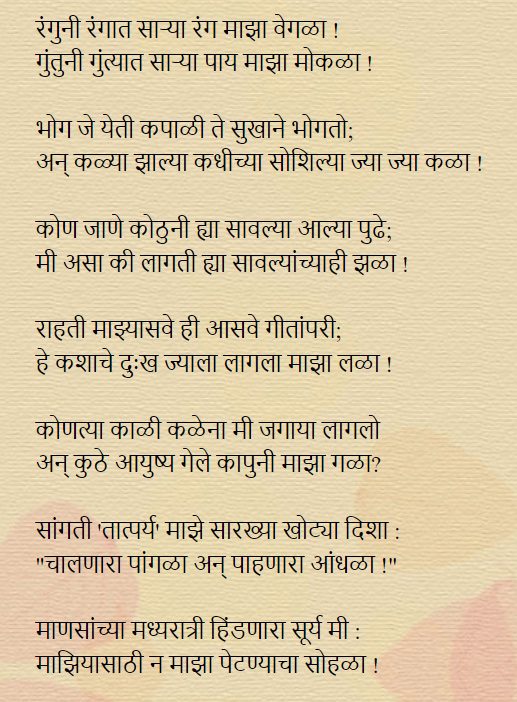
\includegraphics[width=0.4\textwidth]{img/rangunii}
\end{center}

\eng{note: Insert video/playback of Deepa's song}

\eng{note: as the song ends, a new video is shown -- this video has all the team members in our team attire; perhaps the team logo should display in the background.}

bara.mya tara ma.m.daLii, lobha aaheca, to vaa.dhaavaa. jyaa mitra-maitri.nii.mcyaa sahakaaryaa"sivaaya he ajibaata "sakya jhaala.m nasata.m tyaa.mcaa aataa paricaya karuuna gheuuyaa \dots

\eng{(note: Everyone introduces themselves as a first name and a last name, or whatever way they think appropriate.)}
\end{document}
